\documentclass[journal,12pt,twocolumn]{IEEEtran}

\usepackage{setspace}
\usepackage{gensymb}

\singlespacing


\usepackage[cmex10]{amsmath}

\usepackage{amsthm}
\usepackage[utf8]{inputenc}
\usepackage{graphicx}
\usepackage{mathrsfs}
\usepackage{txfonts}
\usepackage{stfloats}
\usepackage{bm}
\usepackage{cite}
\usepackage{cases}
\usepackage{subfig}

\usepackage{longtable}
\usepackage{multirow}

\usepackage{enumitem}
\usepackage{mathtools}
\usepackage{steinmetz}
\usepackage{tikz}
\usepackage{circuitikz}
\usepackage{verbatim}
\usepackage{tfrupee}
\usepackage[breaklinks=true]{hyperref}
\usepackage{graphicx}
\usepackage{tkz-euclide}
\usepackage{epsfig}
\usepackage{}
\usetikzlibrary{calc,math}
\usepackage{listings}
    \usepackage{color}                                            %%
    \usepackage{array}                                            %%
    \usepackage{longtable}                                        %%
    \usepackage{calc}                                             %%
    \usepackage{multirow}                                         %%
    \usepackage{hhline}                                           %%
    \usepackage{ifthen}                                           %%
    \usepackage{lscape}     
\usepackage{multicol}
\usepackage{chngcntr}
\usepackage{float}
\DeclareMathOperator*{\Res}{Res}

\renewcommand\thesection{\arabic{section}}
\renewcommand\thesubsection{\thesection.\arabic{subsection}}
\renewcommand\thesubsubsection{\thesubsection.\arabic{subsubsection}}

\renewcommand\thesectiondis{\arabic{section}}
\renewcommand\thesubsectiondis{\thesectiondis.\arabic{subsection}}
\renewcommand\thesubsubsectiondis{\thesubsectiondis.\arabic{subsubsection}}


\hyphenation{op-tical net-works semi-conduc-tor}
\def\inputGnumericTable{}                                 %%

\lstset{
%language=C,
frame=single, 
breaklines=true,
columns=fullflexible
}
\begin{document}


\newtheorem{theorem}{Theorem}[section]
\newtheorem{problem}{Problem}
\newtheorem{proposition}{Proposition}[section]
\newtheorem{lemma}{Lemma}[section]
\newtheorem{corollary}[theorem]{Corollary}
\newtheorem{example}{Example}[section]
\newtheorem{definition}[problem]{Definition}

\newcommand{\BEQA}{\begin{eqnarray}}
\newcommand{\EEQA}{\end{eqnarray}}
\newcommand{\define}{\stackrel{\triangle}{=}}
\bibliographystyle{IEEEtran}
\providecommand{\mbf}{\mathbf}
\providecommand{\pr}[1]{\ensuremath{\Pr\left(#1\right)}}
\providecommand{\qfunc}[1]{\ensuremath{Q\left(#1\right)}}
\providecommand{\sbrak}[1]{\ensuremath{{}\left[#1\right]}}
\providecommand{\lsbrak}[1]{\ensuremath{{}\left[#1\right.}}
\providecommand{\rsbrak}[1]{\ensuremath{{}\left.#1\right]}}
\providecommand{\brak}[1]{\ensuremath{\left(#1\right)}}
\providecommand{\lbrak}[1]{\ensuremath{\left(#1\right.}}
\providecommand{\rbrak}[1]{\ensuremath{\left.#1\right)}}
\providecommand{\cbrak}[1]{\ensuremath{\left\{#1\right\}}}
\providecommand{\lcbrak}[1]{\ensuremath{\left\{#1\right.}}
\providecommand{\rcbrak}[1]{\ensuremath{\left.#1\right\}}}
\theoremstyle{remark}
\newtheorem{rem}{Remark}
\newcommand{\sgn}{\mathop{\mathrm{sgn}}}
\providecommand{\abs}[1]{\left\vert#1\right\vert}
\providecommand{\res}[1]{\Res\displaylimits_{#1}} 
\providecommand{\norm}[1]{\left\lVert#1\right\rVert}
%\providecommand{\norm}[1]{\lVert#1\rVert}
\providecommand{\mtx}[1]{\mathbf{#1}}
\providecommand{\mean}[1]{E\left[ #1 \right]}
\providecommand{\fourier}{\overset{\mathcal{F}}{ \rightleftharpoons}}
%\providecommand{\hilbert}{\overset{\mathcal{H}}{ \rightleftharpoons}}
\providecommand{\system}{\overset{\mathcal{H}}{ \longleftrightarrow}}
	%\newcommand{\solution}[2]{\textbf{Solution:}{#1}}
\newcommand{\solution}{\noindent \textbf{Solution: }}
\newcommand{\cosec}{\,\text{cosec}\,}
\providecommand{\dec}[2]{\ensuremath{\overset{#1}{\underset{#2}{\gtrless}}}}
\newcommand{\myvec}[1]{\ensuremath{\begin{pmatrix}#1\end{pmatrix}}}
\newcommand{\mydet}[1]{\ensuremath{\begin{vmatrix}#1\end{vmatrix}}}
\numberwithin{equation}{subsection}
\makeatletter
\@addtoreset{figure}{problem}
\makeatother
\let\StandardTheFigure\thefigure
\let\vec\mathbf
\renewcommand{\thefigure}{\theproblem}
\def\putbox#1#2#3{\makebox[0in][l]{\makebox[#1][l]{}\raisebox{\baselineskip}[0in][0in]{\raisebox{#2}[0in][0in]{#3}}}}
     \def\rightbox#1{\makebox[0in][r]{#1}}
     \def\centbox#1{\makebox[0in]{#1}}
     \def\topbox#1{\raisebox{-\baselineskip}[0in][0in]{#1}}
     \def\midbox#1{\raisebox{-0.5\baselineskip}[0in][0in]{#1}}
%
\title{Assignment 3} 
\author{Atla keerthana}
\maketitle
\newpage
\bigskip
\renewcommand{\thefigure}{\theenumi}
\renewcommand{\thetable}{\theenumi}
Download all python codes from 
\begin{lstlisting}
https://github.com/Gayathri1729/SRFP/tree/main/Assignment3
\end{lstlisting}
%
and latex-tikz codes from 
%
\begin{lstlisting}
https://github.com/Gayathri1729/SRFP/tree/main/Assignment3
\end{lstlisting}
%
\section{CONSTR-2.31}
Construct a Quadrilateral ABCD such that $BC =4.5,AC =5.5,CD =5,BD =7,AD=5.5$.
\section{Explanation}
\begin{enumerate}
    \item the given quadrilateral:-
    
    Let the vertices of the quadrilateral $ABCD$ be $\vec{A}$,$\vec{B}$,$\vec{C}$ and $\vec{D}$ .
    
    \item List out given data in form of vectors:-
    
    Given:
    
    $BC =4.5,AC =5.5,CD =5,BD =7,AD=5.5$.
    In vector form,
    \begin{align}
    \norm{\vec{B}-\vec{C}} &= 4.5
    \\
    \norm{\vec{A}-\vec{C}} &= 5.5
    \\
    \norm{\vec{C}-\vec{D}} &= 5
    \\
    \norm{\vec{B}-\vec{D}} &= 7
    \\
    \norm{\vec{A}-\vec{D}} &= 5.5
    \end{align}
    
    \item Find out two triangles of given quadrilateral having same base:
    
    Quadrilateral $ABCD$ is made up of two triangles $\triangle ACD$ and $\triangle BCD$ placed on base $CD$ .
    
\item Verify that construction of both triangles,is possible or not by using the fact that "sum of any two sides of a triangle is greater than the third side":-
   \item[(a)]
Consider $\triangle ACD$,
\begin{align}
    \norm{A-C}+\norm{C-D} &=6.5 >\norm{A-D}\\
    \norm{A-D}+\norm{C-D} &=6.5 >\norm{A-C}\\
    \norm{A-C}+\norm{A-D} &=11 >\norm{C-D}
\end{align}
Sum of any two sides is greater than the third side in $\triangle ACD$ .
 $\therefore$ Construction of $\triangle ACD$ is possible.
\item[(b)]
Similarly in $\triangle BCD$,
\begin{align}
    \norm{B-C}+\norm{C-D} &=9.5 >\norm{B-D}\\
     \norm{B-C}+\norm{B-D} &=11.5 >\norm{C-D}\\
    \norm{B-D}+\norm{C-D} &=12 >\norm{B-C}
\end{align}
Sum of any two sides is greater than the third side in $\triangle BCD$ .
    $\therefore$ Construction of $\triangle BCD$ is possible.
\item Conclude that construction of quadrilateral is possible if both triangles can be constructed otherwise not possible:-
$\because$ both the triangles can be constructed,we can construct the quadrilateral with the given sides.
\item To find the coordinates of the vertices of the given quadrilateral:
Let the sides of the triangles be denoted by $BC=bc,AC=ac,CD=cd,BD=bd,AD=ad$ 
Then,
\begin{equation}
   bc=4.5,ac=5.5,cd=5,bd=7,ad=5.5 
\end{equation}
Suppose $\angle ACD$=N and  $\angle BCD$=M
Now,let
\begin{equation}
   \vec{A}=\myvec{0\\0} \label{eq1}
\end{equation}
\begin{equation}
    \vec{B}=\myvec{5.5\\0} \label{eq2}
\end{equation}
\begin{equation}
     \vec{C}=\myvec{p\\q}=\myvec{i\cos N\\i\sin N} \label{eq3}
\end{equation}
\begin{equation}
    \vec{D}=\myvec{r\\s}=\myvec{t\cos M\\t\sin M} \label{eq4}
\end{equation}
Then we know that,
\begin{align}
  \cos N&=\frac{bc^2+bd^2-ac^2}{2bci}\\
    p&=i\cos N=\frac{bc^2+bd^2-ac^2}{2f}\\
    &=\frac{4.5^2+7^2-5.5^2}{2\times 4.5}=4.33\\
   \sin N&=\pm\sqrt{1-\cos^2 N}\\
   q&=i\sin N=\pm\sqrt{bd^2-bd^2\cos^2 N}\\
   &=\pm\sqrt{7^2-4.33^2}=\pm5.500\\
   \cos M&=\frac{cd^2+bc^2-ad^2}{2bct}\\
  r&= t\cos M=\frac{cd^2+bc^2-ad^2}{2bc}\\
    &=\frac{5^2+4.5^2-5.5^2}{2\times 4.5}=1.66\\
     \sin M&=\pm\sqrt{1-\cos^2 M}\\
  s&= t\sin M=\pm\sqrt{t^2-t^2\cos^2 M}\\
   &=\pm\sqrt{5^2-1.66^2}=\pm4.71
\end{align}
Consider q and s to be positive.Then the coordinates of the quadrilateral can be obtained from \ref{eq1}, \ref{eq2}, \ref{eq3} and \ref{eq4}.
\begin{equation}
\vec{A}=\myvec{0\\0},\vec{B}=\myvec{5.5\\0},\vec{C}=\myvec{4.33\\5.50},\vec{D}=\myvec{1.66\\4.71}
\end{equation}
\item Knowing all the coordinates, now we can construct the quadrilateral.
\numberwithin{figure}{section}
\begin{figure}[!ht]
\centering
    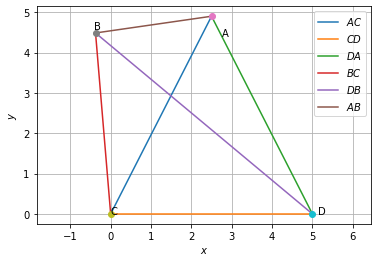
\includegraphics[width= \columnwidth]{quad.png}
    \caption{Quadrilateral $ABCD$}
\end{figure}
\end{enumerate}
\end{document}